\documentclass[
    12pt,                  % Tamanho da fonte do texto
    openright,             % Capítulos começam em páginas ímpares (à direita)
    oneside,               % Impressão apenas em um lado da folha
    a4paper,               % Tamanho do papel (A4)
    chapter=TITLE,         % Estilo dos títulos de capítulos
    section=TITLE,         % Estilo dos títulos de seções
    brazil                 % Idioma principal: português do Brasil
]{abntex2}                 % Classe de documento compatível com normas ABNT

\usepackage[
    alf,
    abnt-emphasize=bf,
    abnt-etal-list=3,
    abnt-full-initials=yes,
]{abntex2cite}

% ----------------------------------------------------------
% Pacotes básicos de formatação
% ----------------------------------------------------------

\usepackage[utf8]{inputenc}      % Suporte para caracteres acentuados (ex: ç, á, ê)
\usepackage[T1]{fontenc}         % Seleção de codificação da fonte para melhorar a hifenização
\usepackage{lmodern}             % Usa a fonte Latin Modern (substituta da Computer Modern)
\usepackage{microtype}           % Melhora a justificação do texto e a microtipografia
\usepackage{graphicx}            % Permite incluir imagens no documento
\usepackage{color}               % Permite o uso de cores (útil para gráficos, seções etc.)
\usepackage{amsmath}             % Pacote da AMS para símbolos e fórmulas matemáticas
\usepackage{hyperref}            % Cria links clicáveis para referências, URLs e sumário
\usepackage{listings}
\usepackage{xcolor} % Para cores personalizadas no código

\usepackage[utf8]{inputenc}
\usepackage[T1]{fontenc}
\usepackage{listings}
\usepackage{xcolor}

\lstdefinelanguage{R}{
  keywords={if, else, repeat, while, function, for, in, next, break},
  otherkeywords={<-, <<-},
  sensitive=true,
  morecomment=[l]\#,
  morestring=[b]",
}

\lstset{
  language=R,
  basicstyle=\ttfamily\small,
  keywordstyle=\color{blue},
  commentstyle=\color{gray}\itshape,
  stringstyle=\color{orange},
  showstringspaces=false,
  numbers=left,
  stepnumber=1,
  numbersep=4pt,
  frame=single,
  captionpos=b
}


% ----------------------------------------------------------
% Pacote de citação conforme normas da ABNT
% ----------------------------------------------------------
% Estilo de citação numérico. Trocar por [alf] para autor-data

% ----------------------------------------------------------
% Informações do trabalho (usadas na capa, folha de rosto etc.)
% ----------------------------------------------------------
\titulo{Minha Opinião Sobre Cinema :\\ Uma visita aos meus filmes favoritos}        % Título do trabalho
\autor{Ingryd França de Sena Melo}                                               % Nome do autor
\local{Fortaleza}                                                   % Local (cidade)
\data{2025}                                                         % Ano
\instituicao{%
  Universidade Federal do Ceará\\                                   % Nome da instituição
  Centro de Ciências - Departamento de Estatística e Matemática Aplicada\\
  Curso de Estatística}
\tipotrabalho{Ensaio Crítico.}                 % Tipo do trabalho
\preambulo{Trabalho apresentado como requisito de nota sobre a disciplina \LaTeX para a cadeira Ferramentas Computacionais.}  % Texto explicativo


% ----------------------------------------------------------
% Início do documento
% ----------------------------------------------------------
\begin{document}

% Gera a capa do trabalho (formato ABNT)
\imprimircapa

% Gera a folha de rosto
\imprimirfolhaderosto

% ----------------------------------------------------------
% Resumo do trabalho
% ----------------------------------------------------------
\begin{resumo}
Este trabalho apresenta minha visão pessoal sobre o universo cinematográfico atual, abordando filmes e séries dos quais assisti e que são os meus favoritos, além de uma breve análise descritíva sobre a Saga dos Vingadores. Busco refletir e opinar sobre as narrativas, a cinematografía, a trilha sonora, o desenvolvimento dos personagens e os aspectos sociais que são usados como base para cada obra citado. Discuto sobre o impacto da arte visual em seu papel de abordar temas relevantes e em como isso me inpactou. Os filmes e séries dos quais vou citar são os quais tiveram mais inpacto em mim, tanto emocional quanto pela história bem construída. Meu objetivo é mostrar como filmes, séries e músicas - junto à arte visual - podem contar histórias, mas também criticar questões sociais de forma profunda.
 \end{resumo}   

\tableofcontents



\chapter*{Introdução}
É notório que a arte sempre teve um grande papel na sociedade, principalmente na forma de contar histórias e criticar a própria humanidade. O cinema nasceu do teatro, que, por sua vez, surgiu da tradição de narrar histórias e poesias. Assim, o objetivo não mudou, apenas se transformou a maneira como é apresentado.\\ \vspace{0.1px}

\noindent A primeira vez que fui ao cinema, assisti a um filme chamado Valente. Esse primeiro contato em uma sala de cinema mudou parte da minha vida: tornou-se um programa em família, que depois se transformou em um passeio entre amigos. Hoje, assistir a filmes, junto com ouvir música e desenhar, é um dos meus hobbies favoritos. Naquela época, eu não entendia como Valente era um filme tão importante, assim como muitos outros que viria a assistir, mas foi o primeiro filme da Disney/Pixar que não focava em uma princesa à procura de um pretendente.\\ \vspace{0.1px}

\noindent Conforme fui crescendo, as idas ao cinema continuaram, e minha paixão por heróis, influenciada pelo meu pai, aumentou quando vi Vingadores: A Era de Ultron no cinema. Hoje, filmes de super-heróis são uma das minhas coisas favoritas. Minha vontade de assistir não se limitou apenas às salas de cinema. Com a chegada dos streamings, ganhei a chance de explorar mais filmes, o que me levou a escrever este breve estudo analítico sobre meus filmes preferidos.\\ \vspace{0.1px}

\noindent Portanto, em amor à arte visual, abordarei meus filmes e algumas séries favoritos, além de uma breve análise descritiva sobre a saga Vingadores.


\chapter*{Saga Vingadores}
\section{Introdução}
O MCU (Universo Cinematográfico da Marvel) é um universo que se estende além dos filmes em que todos os heróis aparecem juntos, abrangendo também os filmes individuais de cada personagem, os quais, quando unidos, criam uma narrativa interconectada. A história segue uma ordem cronológica específica, conforme a lista abaixo:\\
\vspace{0.05cm}\\
-\textit{Capitão América: O Primeiro Vingador (1943 - 1945)\\
-Capitã Marvel (1995)\\
-Homem de Ferro (2008)\\
-Homem de Ferro 2 (2010)\\
-O Incrível Hulk (acontece em paralelo a Homem de Ferro 2, em 2010)\\
-Thor (2011)\\
-Os Vingadores (2012)\\
-Homem de Ferro 3 (2012)\\
-Thor: O Mundo Sombrio (2013)\\
-Capitão América: Soldado Invernal (2014)\\
-Guardiões da Galáxia (2014)\\
-Guardiões da Galáxia Vol. 2 (logo após o primeiro filme, também em 2014)\\
-Vingadores: Era de Ultron (2015)\\
-Homem-Formiga (2015)\\
-Capitão América: Guerra Civil (2016)\\
-Viúva Negra (acontece logo após Guerra Civil, em 2016)\\
-Pantera Negra (2016)\\
-Homem-Aranha: De Volta ao Lar (2016)\\
-Doutor Estranho (2016 - 2017)\\
-Thor: Ragnarok (2017)\\
-Homem-Formiga e a Vespa (acontece antes e durante Vingadores: Guerra Infinita, 2018)\\
-Vingadores: Guerra Infinita (2018)\\
-Vingadores: Ultimato (2018–2023)\\}
\vspace{0.05cm}\\
Essa lista foi pegue do site \cite{marvel2024}, onde tem a ordem cronológica para assistir a todos os filmes. Como são muitos filmes, escolhi trabalhar com apenas os quatro principais - Os Vingadores, Vingadores: a Era de Ultron, Vingadores: Guerra Infinita, Vingadores: Ultimato - para a análise descritiva.
\newpage
\section{Banco de Dados}
Para a análise utilizei alguns sites, como \cite{dados2025} para obter alguns dados e conseguir montar uma planilha usando o Google Sheets e depois usar esses dados no R.

\begin{table}[h]
\centering
\begin{tabular}{|l|r|r|r|r|}
\hline
\textbf{Filmes} & \textbf{Bilheteria(bi)} & \textbf{Aprovação(\%) } & \textbf{Orçamento(mi)} & \textbf{Duração(min)} \\
\hline \hline
The Avengers    & 151 & 91 & 220 & 133.8 \\
Age of Ultron   & 140 & 76 & 444 & 132.6 \\
Infinity War    & 204 & 85 & 400 & 137.4 \\
Endgame         & 279 & 94 & 400 & 186.0 \\
\hline
\end{tabular}
\caption{Resumo financeiro e técnico dos filmes da saga Vingadores.}
\label{tab:vng}
\end{table}
\vspace{0.2cm}
\noindent Esta foi a planilha que fiz com os dados financeiros e técnicos sobre os filmes, buscando juntá-los para que posteriormente colocar esses dados no R em um \textit{data frame} e assim analisá-lo brevemente.

\section{Análise Descritiva}
Utilizando do \textbf{RStudio}, eu calculei as medidas de tendência central e distribuição, fazendo alguns gráficos e também calculando a correlação entre algumas variáveis.

\begin{lstlisting}[language=R]
library(readxl)
file.choose()

rota_dados <- "C:\\Users\\ingry\\Downloads\\dados - avengers.xlsx"

excel_sheets(rota_dados)
Dados <- read_excel(rota_dados)
\end{lstlisting}
\vspace{0.1cm}
Esses códigos permitiram levar minha planilha no Google Sheets para o R e assim transformá-los em um \textit{data frame}, que me possibilitou trabalhar melhor com os dados.

\begin{lstlisting}[language=R]
#Brilheteria
mean(Dados$`Bilheteria bruta em todo o mundo`)
median(Dados$`Bilheteria bruta em todo o mundo`)
sum(Dados$`Bilheteria bruta em todo o mundo`)
var(Dados$`Bilheteria bruta em todo o mundo`)
sd(Dados$`Bilheteria bruta em todo o mundo`)
\end{lstlisting}
Essas funções me mostram quais as medidas centrais e de disperção dos dados.
\newpage
\begin{lstlisting}[label={lst:saidaR}]
> #Brilheteria
> mean(Dados$`Bilheteria bruta em todo o mundo`)
[1] 193.5
> median(Dados$`Bilheteria bruta em todo o mundo`)
[1] 177.5
> sum(Dados$`Bilheteria bruta em todo o mundo`)
[1] 774
> var(Dados$`Bilheteria bruta em todo o mundo`)
[1] 4029.667
> sd(Dados$`Bilheteria bruta em todo o mundo`)
[1] 63.47966
\end{lstlisting}
\begin{lstlisting}[language=R]
#Classificacao
mean(Dados$Classificacao do Rotten Tomatoes)
median(Dados$Classificacao do Rotten Tomatoes)
sum(Dados$Classificacao do Rotten Tomatoes)
var(Dados$Classificacao do Rotten Tomatoes)
sd(Dados$Classificacao do Rotten Tomatoes)
\end{lstlisting}

\begin{lstlisting}[language=R]
#Orcamento
mean(Dados$Orcamento)
median(Dados$Orcamento)
sum(Dados$Orcamento)
var(Dados$Orcamento)
sd(Dados$Orcamento)
\end{lstlisting}

\begin{lstlisting}[language=R]
#Duracao
mean(Dados$Duracao de filme)
median(Dados$Duracao de filme)
sum(Dados$Duracao de filme)
var(Dados$Duracao de filme)
sd(Dados$Duracao de filme)
\end{lstlisting}

\begin{lstlisting}[language=R]
#correlacao linear
cor(Dados$Bilheteria bruta em todo o mundo, 
Dados$Orcamento, method = "pearson")
cor(Dados$Classificacao do Rotten Tomatoes, 
Dados$Bilheteria bruta em todo o mundo, method = "pearson")
\end{lstlisting}
Este arquivo foi criado utilizando o editor \LaTeX, com os pacotes \texttt{listings}, \texttt{xcolor} e \texttt{inputenc} para suportar acentuação e incluir blocos de código em R. O código R foi inserido diretamente no documento com o \texttt{lstlisting}, sem execução automática. Os dados apresentados foram gerados com base em exemplos simples simulados diretamente no script. \\ 
\noindent Essas funções me trouxeram diferentes resultados sobre as variáveis usadas para analisar, como também alguns gráficos interessantes, além de uma ideia de como certas variáveis se correlacionam com outras. 

\begin{figure}[h]
    \centering
    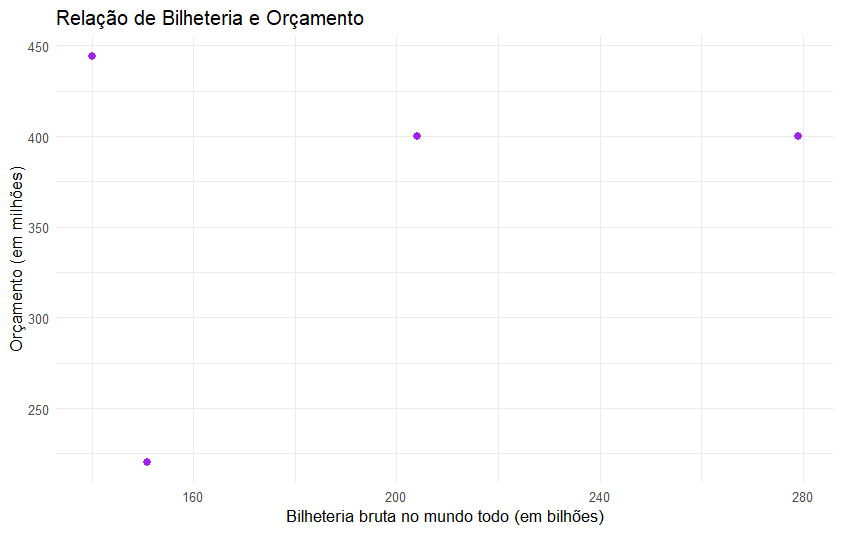
\includegraphics[width=0.70\linewidth]{Disperção_BIlheteria.Orçamento.png}
    \caption{Gráfico de Disperção}
    \label{fig:enter-label}
\end{figure}

\noindent Como visto a alta disperção dos dados de forma não linear se da pelo calculo feito entre as duas variáveis usadas, mostrando que o Orçamento não influência na Bilheteria e virse-versa. Portanto dentre esses quatro filmes usados, a bilheteria não depende do aumento de orçamento na produção, também pela fraca correlação.

\begin{figure}
    \centering
    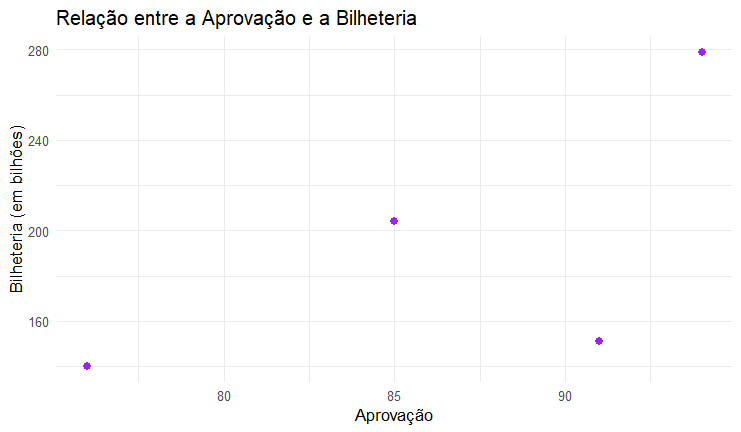
\includegraphics[width=0.70\linewidth]{Disperção_Aprovação.Bilheteria.png}
    \caption{Gráfico de Disperção}
    \label{fig:enter-label}
\end{figure}
\newpage
\noindent No entanto, vemos que existe nesse outro gráfico uma correlação linear maior, mostrando que a aprovação do público influência na bilheteria, podemos notar também que é uma correlação positiva, oque significa que quando maior a aprovação da crítica e do público, maior a bilheteria.

\subsection{Fórmulas de Medidas}
Para calcular manualmente as medidas usadas para a análise aqui estão as usadas: \\
\vspace{0.3cm}

\textbf{Média}:
\begin{equation}
\bar{x} = \dfrac{1}{n}\sum_{i=1}^{n} x_{i}
\label{eq:media}
\addcontentsline{toc}{subsection}{Equação \theequation: Média Aritmética}
\end{equation}

\textbf{Mediana}:
\begin{equation}
\text{md}(X) =
\begin{cases}
x_{\left( \frac{n+1}{2} \right)}, & \text{se } n \text{ for ímpar} \\
\dfrac{x_{\left( \frac{n}{2} \right)} + x_{\left( \frac{n}{2} + 1 \right)}}{2}, & \text{se } n \text{ for par}
\end{cases}
\label{eq:mediana}
\addcontentsline{toc}{subsection}{Equação \theequation: Mediana}
\end{equation}

\textbf{Soma}:
\begin{equation}
\sum_{i=1}^n x_i
\label{eq:soma}
\addcontentsline{toc}{subsection}{Equação \theequation: Soma}
\end{equation}

\textbf{Variância}:
\begin{equation}
s^2 = \dfrac{1}{n - 1} \sum_{i=1}^{n} (x_i - \bar{x})^2
\label{eq:variancia}
\addcontentsline{toc}{subsection}{Equação \theequation: Variância}
\end{equation}

\textbf{Desvio-padrão}:
\begin{equation}
s = \sqrt{ \dfrac{1}{n - 1} \sum_{i=1}^{n} (x_i - \bar{x})^2 }
\label{eq:desviopadrao}
\addcontentsline{toc}{subsection}{Equação \theequation: Desvio padrão}
\end{equation}

\textbf{Correlação linear}:
\begin{equation}
\text{corr}(x, y) = \dfrac{ \sum_{i=1}^{n} (x_i - \bar{x})(y_i - \bar{y}) }{ \sqrt{ \sum_{i=1}^{n} (x_i - \bar{x})^2 } \sqrt{ \sum_{i=1}^{n} (y_i - \bar{y})^2 } }
\label{eq:correlacao}
\addcontentsline{toc}{subsection}{Equação \theequation: Correlação}
\end{equation}

\noindent Essas fórmulas podem ser encontradas no livro \cite{Bussab2017Cap3}, de Estatística Básica, usado no primeiro semestre de Estatística.

\newpage
\section{Gráficos}
Aqui alguns gráficos de frequência sobre as variáveis usadas.\\
\begin{figure}[h]
    \centering
    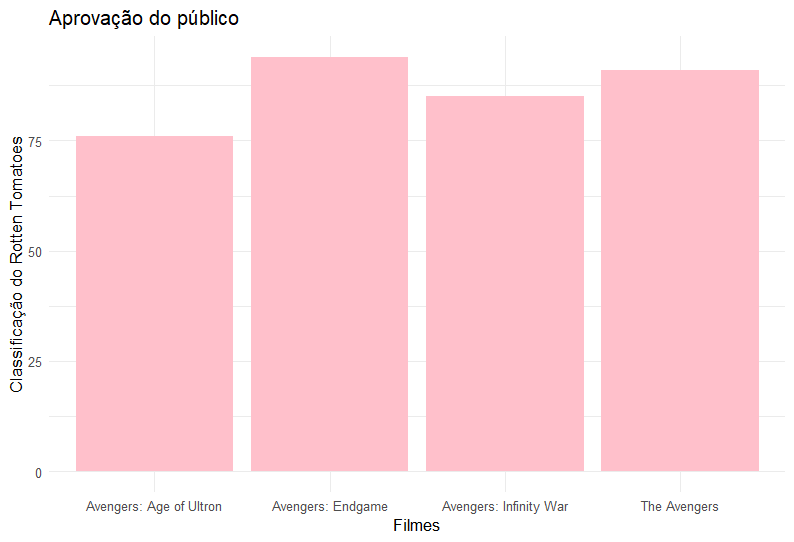
\includegraphics[width=0.55\linewidth]{Bar_Aprovação.png}
    \caption{Aprovação}
    \label{fig:enter-label}
\end{figure}
\begin{figure}[h]
    \centering
    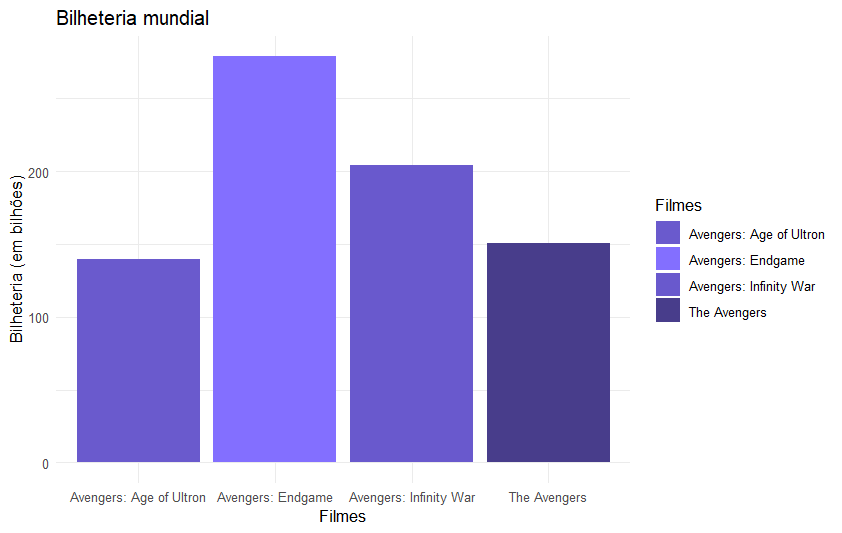
\includegraphics[width=0.65\linewidth]{Bar_Bilheteria.png}
    \caption{Bilheteria}
    \label{fig:enter-label}
\end{figure}
\begin{figure}[h]
    \centering
    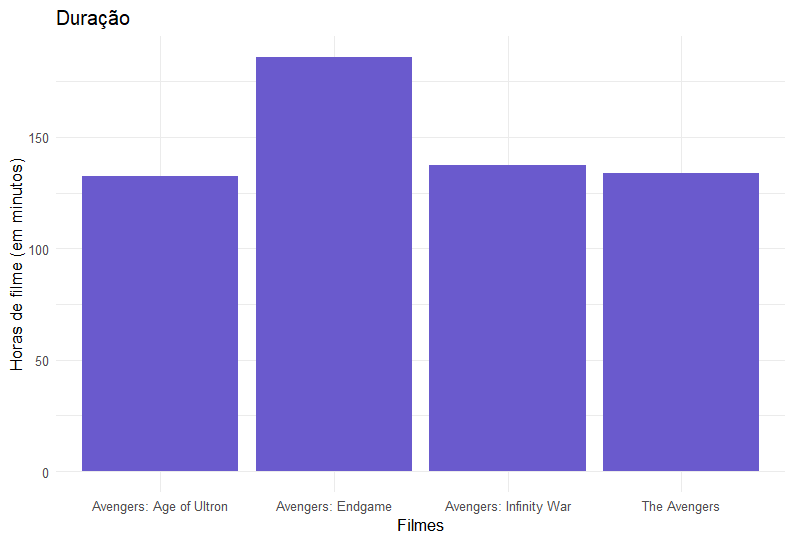
\includegraphics[width=0.55\linewidth]{Bar_Duração.png}
    \caption{Duração}
    \label{fig:enter-label}
\end{figure}
\begin{figure}[h]
    \centering
    \includegraphics[width=0.55\linewidth]{Bar_Orçamento.png}
    \caption{Orçamento}
    \label{fig:enter-label}
\end{figure}\newpage
\noindent O livro \cite{Bussab2017}, ajudou muito a compreender os conteúdos necessários para tal análise, como medidas centrais e de disperção, além de gráficos e assimetría, é recomendado lê-lo caso a análise tenha capturado sua atençaõ.
\newpage
\section{Opinião}
A Saga Vingadores marcou bastate minha infância e adolescência, e até hoje continuo assistindo aos filmes. Ao reassistir Os Vingadores, percebo pequenos detalhes que antes haviam passado despercebidos ou que não compreendia. Um exemplo é o personagem Loki: na primeira exibição, não tínhamos o contexto completo sobre esse "vilão", que depois descobrimos ser manipulado por uma entidade maior – Thanos, como viríamos a conhecer mais tarde.\\ \vspace{0.1px}

\noindent É incrível como, antes mesmo do lançamento do filme principal, a Marvel criou filmes individuais para apresentar cada um dos heróis originais, criando assim a atmosfera perfeita para o encontro do grupo. A direção mostra bastante criatividade em diversas cenas, principalmente nas sequências de luta do ato final. A fotografia, embora não seja inovadora – seguindo um estilo clássico da Marvel –, funciona muito bem para o universo que estava sendo construído, por transmitir a sensação de que aquele mundo poderia ser o nosso. \\ \vspace{0.1px}

\noindent As dinâmicas entre os personagens são interessantes. As piadas funcionam com naturalidade, e os conflitos internos são bem desenvolvidos, plantando sementes para eventos futuros, como em \textit{Capitão América: Guerra Civil}, cujas consequências ecoam até Ultimato.\\ \vspace{0.1px}

\noindent Ao longo da saga, observamos um notável desenvolvimento dos personagens, com destaque especial para o Homem de Ferro, que acaba por roubar a cena nessa fase. Outros personagens também recebem arcos em seus filmes solo – Loki, Thor, Homem-Aranha, Falcão, Viúva Negra, Doutor Estranho, Capitão América e Hulk –, cada um com uma evolução diferente. No entanto, o crescimento de Tony Stark é particularmente marcante: de um playboy egoísta, ele se transforma na própria definição de herói.\\ \vspace{0.1px}

\noindent Em Ultimato, vemos um Tony Stark diferente daquele apresentado no primeiro filme dos Vingadores. Sua decisão de ajudar os companheiros a voltar no tempo – motivada por ter perdido Peter Parker no "estalo" – contrasta com o egoísmo que era bem visível no passado, quando provavelmente teria priorizado sua família e felicidade pessoal.\\ \vspace{0.1px}

\noindent O clímax do filme se dá na batalha final contra Thanos. Embora emocionante, a sequência poderia ter sido melhor dirigida, já que em alguns momentos transmite uma certa sensação de vazio no campo de batalha. Ainda assim, há cenas memoráveis, especialmente o clímax, quando Tony Stark profere sua frase marcante – um momento que fecha o ciclo iniciado no primeiro Homem de Ferro e consagra para sempre o legado do personagem e da Saga.\\

\begin{quote} \center
    "Eu sou o Homem de Ferro."
\end{quote}
\flushleft

No geral, a Saga Vingadores é muito boa, mas reconheço que parte de seu sucesso se deve ao momento bom para filmes de heróis na época. Atualmente, a Marvel parece tentar recriar esse mesmo ânimo e manter a conexão entre seus filmes em um universo compartilhado. No entanto, terão um grande desafio se quiserem repetir o fenômeno cultural que eles mesmos criaram, pois o apelo dos heróis parece estar diminuindo - mesmo que, aparentemente, \textit{Superman (2025)} tenha feito um excelente trabalho ao reacender esse entusiasmo.


\chapter*{La La Land: Cantando Estações}
La La Land é um musical que conta a história de Sebastian, um pianista de jazz, e Mia, uma aspirante a atriz, que se conhecem e se apaixonam em Los Angeles. Dirigido e escrito por Damien Chazelle, o filme é um musical de romance. Posso dizer que não sou muito fã de romances ou musicais, mas o fato de ter vencido o Oscar despertou minha curiosidade – assim como a trilha sonora, que inclui uma de minhas músicas favoritas, \textit{City of Stars}. Então, pela premiação, decidi assistir e rapidamente se tornou um dos meus filmes preferidos. Entre os muitos motivos, destacam-se a fotografia impecável (uma marca registrada de Chazelle) e o final não tão comum em filmes de romance. \\ 
\vspace{13px}
\noindent A maneira como a iluminação e as cores transformam cada cena em algo incrível foi algo que me conquistou. No entanto, o que aumentou meu amor pelo filme foi a escolha do final: os protagonistas não ficam juntos. Essa decisão, acrescentou uma profundidade à história e aos próprios personagens. \\ \vspace{0.1px}
\vspace{13px}
\noindent Mesmo um considerável tempo despois de assistir, ainda reflito sobre sua mensagem. O romance entre Mia e Sebastian é construído devagar, até o momento em que uma discussão os separam. O que mais me marcou é a cena em que Sebastian, mesmo após o afastamento, recebe uma ligação em sua casa - pois antes eles moravam juntos - sobre uma audição importante para Mia e vai até ela para incentivá-la a fazer a audição. Isso me fez notar que o filme não é apenas sobre amor romântico, mas também sobre a paixão pelos próprios sonhos – o que os motiva a continuar. \\ \vspace{0.1px}
\vspace{13px}
\noindent Essa é, para mim, a mensagem do filme. Mia realiza seu sonho de se tornar atriz, e Sebastian abre seu tão desejado clube de jazz. Eles se amavam, mas sabiam que seus caminhos eram diferentes. Em vez de se anularem pelo relacionamento, escolheram seguir seus sonhos. A mensagem clara de que sonhar, lutar pelo que ama e não desistir. O romance serve como pano de fundo para essa lição, que acentua perfeitamente com a música  \textit{City of Stars}. \\ 



\chapter*{Pecadores}
Pecadores (ou Sinners) foi lançado este ano e rapidamente conquistou o posto de meu filme favorito. Dirigido por Ryan Coogler e estrelado por Michael B. Jordan no papel principal, atuando como gêmeos, a narrativa se passa em uma época marcada pelo racismo, usando a figura dos vampiros como uma metáfora para a apropriação cultural – especialmente da cultura negra. \\ 
\vspace{13px}
\noindent O que mais me impressionou, além da direção impecável e das  boas atuações, foi a mensagem, presente em cada cena. Os vampiros, mais do que criaturas para adcionarem terror e trama na história, simbolizam a forma como a história e as tradições são "roubadas". A maneira como o filme explora essa ideia – mostrando que essas criaturas não apenas só um perigo. \\ 
\vspace{13px}
\noindent A estrutura é genial, uma cena inicial visualmente comum ganha um peso quando revista no final, agora com todo o contexto que faltava. A ancestralidade e a cultura são tratadas com tanto cuidado que cada detalhe, desde as expressões dos personagens até as escolhas da trilha sonora, contribui para uma experiência cinematográfica. Falando em música, a trilha não está ali apenas como fundo, mas como parte da narrativa, complementando a atuação de forma única. \\ 
\vspace{13px}
\noindent O final agridoce deixa o filme único – não por ser incompleto, mas por criar um universo tão cru e real. A mistura de gêneros – terror, ação e drama musical – faz de Pecadores não apenas um dos melhores filmes de 2025, mas uma obra que ressoa muito além da tela e pode ser necessária nos dias de hoje.

\chapter*{Outros}
Alguns filmes e séries merecem destaque, mesmo que brevemente:\\
\vspace{16px}
- Barbie (2023): Um filme que curou minha criança interior. Além de me fazer rir e chorar, adorei a originalidade e coragem em ser exatamente o que é. O discurso final, por mais óbvio que pareça, sempre me faz refletir, e a composição musical do clímax é emocionante, junto as montagens de imagens da infância. \\
\vspace{12px}
- Homem-Aranha no Aranhaverso (2018/2023): Uma obra-prima visual. Como alguém que ama desenhar, fico fascinada com a forma como cada universo tem seu próprio estilo de animação, mantendo a essência única de seus personagens, mesmo quando eles estão em universos diferentes. Cada frame é feito com tanto cuidado que parecem pinturas da arte.\\
\vspace{12px}
- Duna – Parte 1 e 2 (2021/2024): Um espetáculo de fotografia. Denis Villeneuve conseguiu criar o antes impossível mundo de Duna com maestria, como o planeta Harkonnen em preto e branco quando o Sol negro brilha fora de lugares cobertos, contrastando com os desertos de Arrakis. A atuação de Timothée Chalamet é excepcional, embora a personagem Chani (Zendaya) merecesse mais desenvolvimento. Ainda assim, uma das melhores experiências cinematográficas recentes.\\
\vspace{12px}
- Harry Potter (Saga): Reconheço seus defeitos – desde falhas no roteiro até escolhas de direção –, mas o mundo mágico criado, marcou minha infância e permanece sendo um filme conforto para mim. O apego emocional aos primeiros filmes, me faz sempre adorar cada um.

Séries que também amo (e recomendo):\\
\textit{- Fleabag,\\
- The Office,\\
- The Bear,\\
- Ruptura.\\}
\vspace{12px}
Cada uma dessas obras, à sua maneira, deixou uma marca – seja pela técnica, pela emoção ou pura diversão.Cada um dos filmes e séries abordam temas diferentes dos 
quais não irei me extender para não tornar o trabalho maior ainda. \\

\chapter*{Conclusão}
A realização deste trabalho permitiu consolidar conhecimentos importantes sobre medidas estatísticas fundamentais, como média, mediana, moda, variância, desvio padrão e correlação linear. A prática com os conceitos matemáticos possibilitou uma compreensão mais profunda sobre sua aplicação e interpretação no contexto de análise de dados.\\
\vspace{13px}
\noindent Durante a execução do trabalho, um dos desafios enfrentados foi a correta formatação das fórmulas matemáticas utilizando o ambiente LaTeX, especialmente no uso de diferentes modos de escrita, como fórmulas em linha e ambientes de equação numerada.\\
\vspace{13px}
\noindent A base bibliográfica foi construída a partir de livros-texto clássicos de Estatística, materiais didáticos disponibilizados por docentes e fontes confiáveis da internet, como artigos acadêmicos e manuais de LaTeX. Essa diversidade de fontes garantiu uma abordagem teórica sólida e ao mesmo tempo prática.\\
\vspace{13px}
\noindent Em suma, os filmes vão muito além do entretenimento: eles têm o poder de transmitir valores, provocar reflexões e fortalecer laços sociais por meio das histórias que contam. Ao abordar temas humanos, culturais e sociais. Como alguns dos filmes que citei é possível ver que tanto assuntos importante são abordados como também o ponto de vista do crescimento de um personagem. Refletir sobre isso reforça a ideia de que contar histórias é uma necessidade essencial do ser humano — e os filmes são, hoje, uma das formas mais impactantes de fazer isso. \\
\vspace{13px}
Recomendo ler o livro \cite{Eisenstein2002}, e \cite{Cinema}, um artigo muito interessante.



\bibliography{Referencias}
\end{document}